\chapter{Anwendung des Pointingmodells auf Daten des Teleskops}
Um das in Kapitel 3 entwickelte Pointingmodell zu testen, wurde mit dem Prototyp des MST ein Datensatz aufgenommen um die Daten
\section{Datensatz}
Der verwendete Datensatz wurde am MST-Prototyp in Adlershof in der Nacht vom 4. auf den 5. Juli 2018 im Zeitraum von 21:00 UTC bis 1:45 UTC aufgenommen. Dazu wurden 105 Postionen beobachtet wobei das Teleskop anfangs Richtung Zenit stand und sich dann in einer abwärtslaufenden Spirale befand. An jeder Position wurden 4 Bilder aufgezeichnet, wovon zwei eine Belichtungszeit von 20 Sekunden hatten. Die jeweils zweiten Bilder mit dieser Belichtungszeit aufgenommenen Bilder wurden verwendet um mithilfe einer Software die Koordinaten des Bildmittelpunktes zu bestimmen. Das war bei 100 Bildern erflolgreich. Der zur Analyse verwendete Datensatz besteht somit aus 100 Einträgen, die jeweils die Elevations und Azimutkoordinaten des Drivesystems (also der am Teleskop eingestellten Koordinaten) und der tatsächlichen (also der Koordinaten des Bildmittelpunktes).
\section{Programm}
Um das Pointingmodell auf Konsistenz zu überprüfen wurde ein Programm in ROOT geschrieben, welches die Differenzen der vom Pointingmodell (Index P) bestimmten Werte mit den gemessenen (Index M) Werten berechnet und analysiert. Da die oben entwickelten Pointingmodelle noch freie Parameter haben, die vom Teleskop abhängen werden diese durch eine Regression der Daten bestimmt. Da das Pointingmodell aus zwei Funktionen besteht (jeweils eine für die Elevation und den Azimut), die jedoch von den gleichen Parametern abhängen, muss hier ein kombinierter Fit durchgeführt werden. Dazu wird eine Hilfsvariable eingeführt, die die Summe der Quadrate der Differenzen von Messwerten und vorhergesagten Werten für feste Werte der freien Parameter bestimmt.
\begin{equation}
Q=\sum^N_{i=1}\left(P_i-M_i\right)^2
\end{equation}
Durch die Bildung der Quadrate können sich Abweichungen nach oben und unten nicht gegenseitig kompensieren und die Hilfsvariable ist somit ein Maß für die Abweichung von Modell mit den gewählten Parametern und Messwerten. Die besten Parameter erhält man, indem man die Variable minimiert. Dazu wurde die in ROOT integrierte Funktion TMinuit verwendet, die zudem noch die Standardabweichung der Parameter ausgibt. Um die Güte des Modells bestimmen zu können wird noch die Größe $\frac{\chi^2}{doF}$ verwendet um die Fehler der Messwerte zu bestimmen, in denen das Modell mit dem Datensatz übereinstimmt. Die Größe $\frac{\chi^2}{doF}$ ist definiert als
\begin{equation}
\frac{\chi^2}{doF}=\sum^N_{i=1}\frac{\left(P_i-M_i\right)^2}{\sigma_i^2}
\end{equation}
wobei hier $\sigma_i$ der Fehler des Wertes i ist und $doF$ der Anzahl der Freiheitsgraden entspricht. Diese berechnet sich durch
\begin{equation}
doF=N-\textrm{Anzahl der Parameter}
\end{equation}
Der perfekte Wert für $\frac{\chi^2}{doF}$ ist 1. Unter der Anahme, dass die Fehler $\sigma$ alle gleich groß sind, lassen sich diese wie folgt berechnen
\begin{equation}
\sigma=\sqrt{\sum^N_{i=1}\left(P_i-M_i\right)^2}=\sqrt{Q}
\end{equation}
Interessant ist es auch, sich die Korrelation der Parameter untereinander anzugucken. Die Korrelation beschreibt die Beziehung der zwischen einzelnen Parametern. Hier wird dazu der Korrelationskoeffizient nach Pearson verwendet, der ausschließlich die lineare Korrelation berücksichtigt. Um diesen zu berechnen wird zunächst die Korelationsmatrix
\begin{equation}
COV(X,Y)=\left<\left(X-\left<X\right>\right)\cdot\left(Y-\left<Y\right>\right)\right>
\end{equation}
berechnet. Auf der Hauptdiagonale stehen die Varianzen, aus denen sich die Fehler der Parameter bestimmen lassen:
\begin{equation}
\sigma_X=\sqrt{COV(X,X)}=\sqrt{VAR(X)}
\end{equation}
Der Korrelationskoeffizient lässt sich nun durch
\begin{equation}
\rho_{XY}=\frac{COV(X,Y)}{\sigma_X\sigma_Y}
\end{equation}\\
Um die Qualität der jeweiligen Pointingmodelle beurteilen zu können, werden jeweils vier Plots ausgegeben, die die jeweiligen Differenzen der bestimmten und gemessenen Koordinaten angeben
\begin{equation}
f=el_M-el_P \quad \textrm{bzw} \quad f=az_M-az_P
\end{equation}
\section{Anwendung auf das Pointingmodell mit 2 Parametern}
Zunächst wird das Modell mit den Parametern $el0$ und $az0$ untersucht.
\subsection{Abhängigkeit der Drivekoordinaten in Abhängigkeit der CCD-Koordinaten}
\begin{figure}[htbp]
\centering
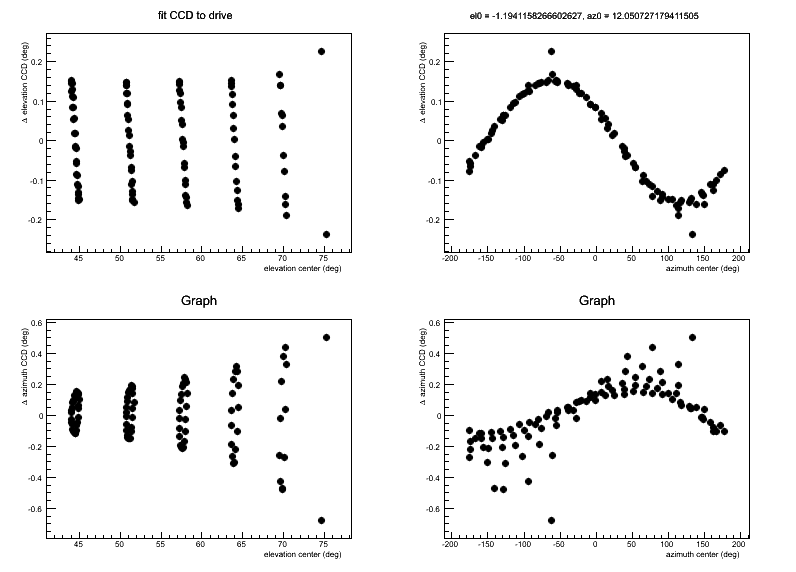
\includegraphics[width=\textwidth]{../341/run341C2D.png}
\caption{Die Drivekoordinaten in Abhängigkeit der CCD-Koordinaten}
\label{img:C2D}
\end{figure}
\subsection{Abhängigkeit der CCD-Koordinaten in Abhängigkeit der Drivekoordinaten}
\begin{figure}[htbp]
\centering
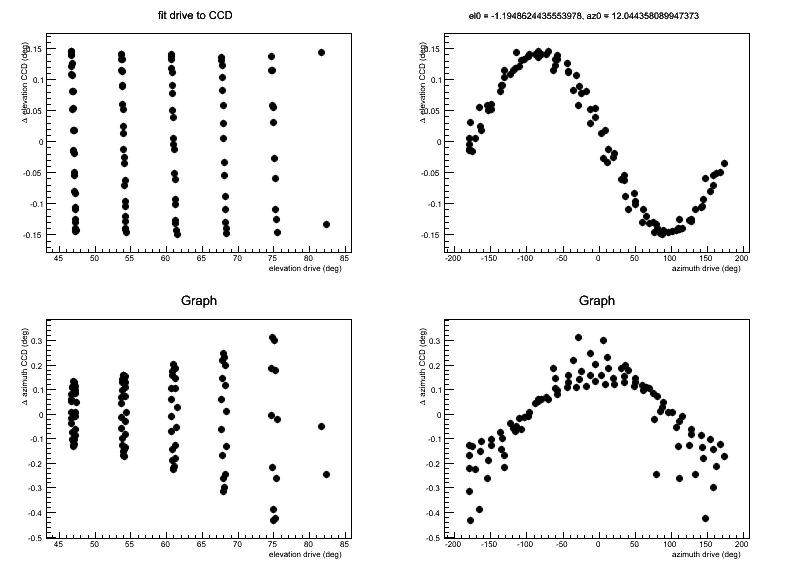
\includegraphics[width=\textwidth]{../341/run341D2C.png}
\caption{Die CCD-Koordinaten in Abhängigkeit der Driveoordinaten}
\label{img:D2C}
\end{figure}

\section{Anwendung auf das Pointingmodell mit 4 Parametern}
\subsection{Abhängigkeit der Drivekoordinaten in Abhängigkeit der CCD-Koordinaten}
\centering
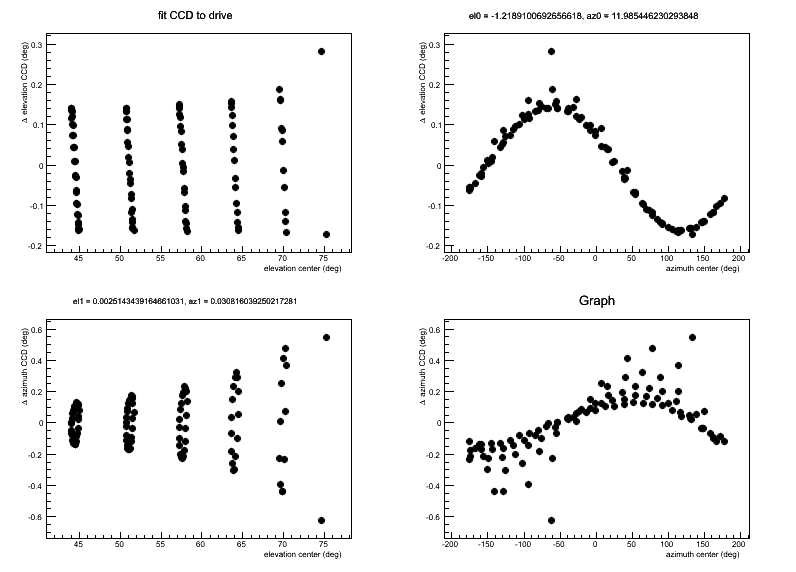
\includegraphics[width=\textwidth]{../341/run341C2D_4par.png}
\caption{Die Drivekoordinaten in Abhängigkeit der CCD-Koordinaten}
\label{img:C2D4}
\end{figure}
\subsection{Abhängigkeit der CCD-Koordinaten in Abhängigkeit der Drivekoordinaten}
\begin{figure}[htbp]
\centering
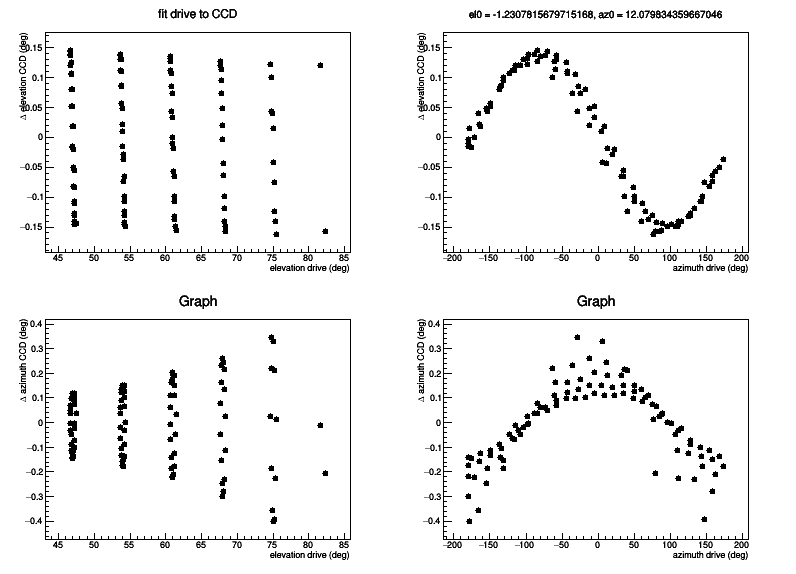
\includegraphics[width=\textwidth]{../341/run341D2C4.png}
\caption{Die CCD-Koordinaten in Abhängigkeit der Driveoordinaten}
\label{img:D2C4}
\end{figure}